\documentclass{article}

% Things to import:
\usepackage{tikz}
\usetikzlibrary{trees,arrows,positioning, calc}
\tikzstyle{redVertex}  =[draw,fill=red,     circle,minimum size=18pt,inner sep=0pt, text=white]
\tikzstyle{blackVertex}=[draw,fill=black,   circle,minimum size=18pt,inner sep=0pt, text=white]
\tikzstyle{nil}        =[draw,fill=black,rectangle,minimum size=18pt,inner sep=0pt, text=white]


\begin{document}
% Used to export it as an image too: (Sourcecode is from here: https://tex.stackexchange.com/a/299008)
\hoffset=-1in\voffset=-1in\setbox0\hbox{


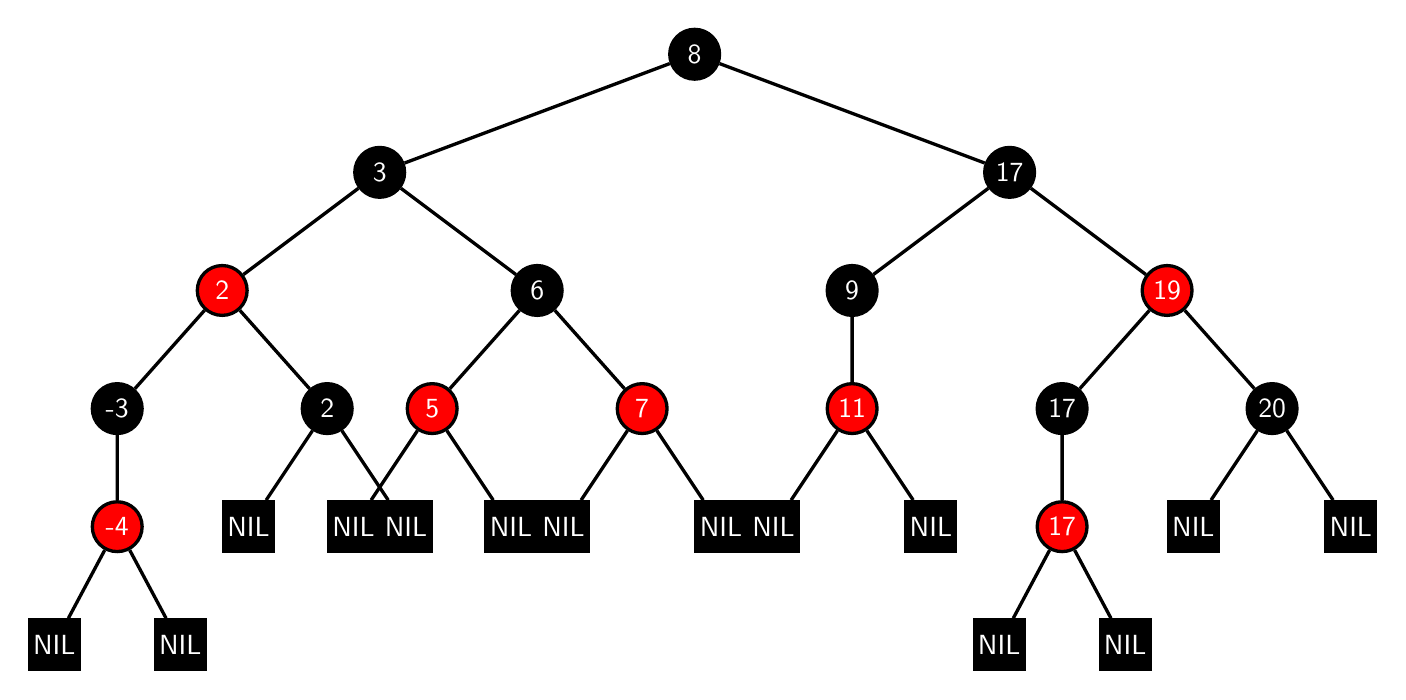
\begin{tikzpicture}[font=\sffamily,very thick,level/.style={sibling distance=80mm/#1}]
\node [blackVertex] (r){8}
child {
	node [blackVertex] {3}
	child {
		node [redVertex] {2}
		child {
			node [blackVertex] {-3}
			child {
				node [redVertex] {-4}
				child {node [nil] {NIL}}
				child {node [nil] {NIL}}
			}
		}
		child {
			node [blackVertex] {2}
			child {node [nil] {NIL}}
			child {node [nil] {NIL}}
		}
	}
	child {
		node [blackVertex] {6}
		child {
			node [redVertex] {5}
			child {node [nil] {NIL}}
			child {node [nil] {NIL}}
		}
		child {
			node [redVertex] {7}
			child {node [nil] {NIL}}
			child {node [nil] {NIL}}
		}
	}
}
child {
	node [blackVertex] {17}
	child {
		node [blackVertex] {9}
		child {
			node [redVertex] {11}
			child {node [nil] {NIL}}
			child {node [nil] {NIL}}
		}
	}
	child {
		node [redVertex] {19}
		child {
			node [blackVertex] {17}
			child {
				node [redVertex] {17}
				child {node [nil] {NIL}}
				child {node [nil] {NIL}}
			}
		}
		child {
			node [blackVertex] {20}
			child {node [nil] {NIL}}
			child {node [nil] {NIL}}
		}
	}
};
\end{tikzpicture}


}\pdfpageheight=\dimexpr\ht0+\dp0\relax\pdfpagewidth=\wd0\shipout\box0\stop